\chapter{Conclusion and Further Work}
\section{Conclusion}
In this thesis we have given an overview of agent solutions used in the manufatcturing world. We found that a gap lies in the ``real'' negotiation, which excludes the use of auctions and or contract net protocol. 

By using the alternating offer protocol it is checked whether an optimal solution can be found. 

At the moment, it seems as if the reactive concession strategy, as described in \citet{zheng2015automated} still has some difficulties. This can be clearly seen in \Cref{fig:reactivevsnon-reactive}. 

\section{Discussion}
Although the alternating offer has been used, it is not usable at al yet at a real case. The largest difficulty lies in the realistic portrayal of the utility function. The requirement for a convex utility function makes it even more difficult. However, if only the non-reactive strategy was used, it should be possible to use a non-convex function.

\todo[Principled Negotiation]{Principled negotiation}

\todo[Far from the optimal as dicussed in the Literature]{Far from the optimal as dicussed in the Literature}
\section{Further research}
A lot of further research could be done on the alternating offer protocol to be used in manufacturing world. The agents could be improved to allow reasoning, using an holonic structure for example. Furthermore other strategies can be used, while the utility functions can be changed as well. Extra negotiation could be applied using bilateral negotiations, and to finalize heuristic learning methods can be applied.

\subsection{Holonic agents}

This structure is that of a holon as can be seen in figure~\cref{fig:holonexample}. As shown in the literature it is based on PROSA by \citet{van1998reference}.
\begin{figure}
	\centering
	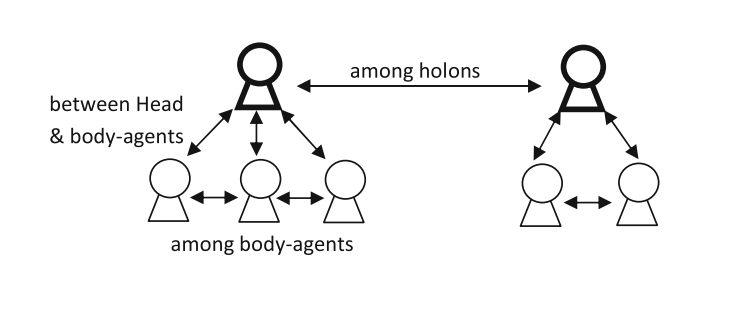
\includegraphics[width=0.7\linewidth]{img/holon_example}
	\caption{An example of the different negotiation between holons from \citet{beheshti2016negotiations}.}
	\label{fig:holonexample}
\end{figure}

The following facts and rules are part of the Anion.

\begin{enumerate}
	\item
	Knowledge of anion head about the sub-agents:
	\begin{itemize}
		\item {$\{A_1, ..., A_6\}$ can process $a$ amount of water}
		\item {$\{A_1, ..., A_6\}$ needs to be cleaned after $b$ water}
		\item {$\{A_1, ..., A_6\}$ has filtered $c$ amount of water}
		\item {$\{A_1, ..., A_6\}$ needs $d$ base to clean}
		\item {$\{A_1, ..., A_6\}$ needs $e$ time to clean}
	\end{itemize}
	\item
	Currently $x$ amount of water being filtered 
	\item
	Currently $Z \subseteq \{A_1, ..., A_6\}$ filter being used for water filtering
	\item
	Currently $Y \subseteq \{A_1, ..., A_6\}$ filter being used for cleaning
	\item
	Currently $w$ amount of base being used for cleaning
\end{enumerate}

\begin{figure}[h]
	
	\centering
	\begin{tikzpicture}
	
	\node[circle,draw,  minimum size=1cm] (A1) at  (0,0) {A$_1$};
	\node[circle,draw,  minimum size=1cm] (A2) at  (0,-1.5) {A$_2$};
	\node[circle,draw,  minimum size=1cm] (A3) at  (0,-3) {A$_3$};
	\node[circle,draw,  minimum size=1cm] (A4) at  (0,-4.5) {A$_4$};
	\node[circle,draw,  minimum size=1cm] (A5) at  (0,-6) {A$_5$};
	\node[circle,draw,  minimum size=1cm] (A6) at  (0,-7.5) {A$_6$};
	%\draw  (0,-2.5) ellipse (1 and 3.4);
	
	\node[ellipse,  draw, minimum height =9cm, minimum width = 2.5cm ] (A) at (0,-3.75) {Anion};
	
	\end{tikzpicture}
	\caption{Anion head and sub-agents}
	\label{fig:anion-head-sub}
	
\end{figure}
The use of these holons could allow an agent to reason about the environment, and act upon it accordingly.

\subsection{Utility function}
The requirement of a convex function forced the use of a specific, and highly theoretical function. This could be perfected using more expert input.
\subsubsection{Reservation curve}
We have used a linear reservation curve for simplicity, since this eliminated the minimization that would have been necessary if a truly curved function was used. An example is shown in \Cref{fig:anionreservationfunction}.
\begin{figure}
	\centering
	\begin{tikzpicture}[domain=0.15:4]
	%\draw[very thin,color=gray] (0.01,0.01) grid (3.9,3.9);
	\draw[->] (0.02,0) -- (4.2,0) node[below] {$Water$};
	\draw[->] (0,0.02) -- (0,4.2) node[left] {$Base$};% node[pos=0.25, left] {$200 m^3 / hr$};
	\draw[color=black] plot (\x,{0.07*exp(\x)}) node[left] {$R_A$};
	\end{tikzpicture}
	\label{fig:anionreservationfunction}
	\caption{The reservation function for the Anion filter: the more water is filtered and given, the more base it requires.}
\end{figure}

\subsection{Continue negotiation after group agreement}
After the group has an agreement, the agents now allocate the resource as predefined (see \Cref{sec:design:mean}). This could be optimized to bilateral negotiation between the Mixbed and Anion for example.
\subsection{Extra concession strategies}
The many concession strategies, as shown in \Cref{sec:concessionstrat} allow for many strategies to be used. Further research could include using fraction, which was suggested as a good solution by \citet{wu2009efficient}. 
\subsection{Heuristic learning methods}
As shown in \Cref{sec:lit:learn}, heuristic learning methods can also be used to learn the desired utility function. This has not been done since the requirement of a convex utility functions forced the usage of predefined functions.
\todos
